\section{Implementation}
\label{sec:implementation}

The proposed service consists of several aspects: an interface for tablet computers; web-based streaming of video; programme recommendations; advert campaigns and management functionality; advert selection processes; and the general architecture of the hardware and interfaces that tie the system together.

In the following section, the technical details of the implemented system, \textit{Your4.tv}, will be discussed. This includes the overall systems architecture, database design, and the languages and tools used during the development process.

\subsection{Requirements elicitation}
In order to ensure the completion of the project in the limited time available the requirements were discussed with respect to the benefit to each of the stakeholder and then subdivided using the MoSCoW system developed as part of \citet{clegg1994case}.

\subsubsection{Stakeholders}
\begin{description}
\item[Advertisers:]{With the increasing audience fragmentation discussed in \ref{sec:evolution_of_TV} the cost of advertising relative to its effectiveness is dramatically rising. If this project is a success, advertisers will be able to create an advertising campaign that operates over a range of channels, targeting audience members specifically - rather than spreading their advertising over a number of channels and hoping that it reaches the appropriate audience. This will reduce the overal cost of advertising to viewers, as the process can be more efficient. Additionally, by adding rich interaction to TV adverts our platform will supply the tools to allow TV advertisers to improve user engagement and provide incentive to keep attention on their adverts.}
\item[Broadcasters:]{With the considerable increase in granularity provided by our proposed system, over the usual programme context and timings, the advert space value for a broadcaster using this system would be greatly improved and give a far better return on investment. Especially with the additional options of providing interactive elements for their adverts, advertisers are likely to pay more for less time, meaning that the return on investment for the broadcaster is significantly improved. In addition our system's compatibility with tablet devices may increase the market share for broadcasters using this service over those who do not.}
\item[Users:]{\citet{broadcastEconomics} states that users have a symbiotic relationship with adverts where adverts are made palatable by the content surrounding them. Within our system the addition of interactivity to adverts means that advertisers will be able to provide entertainment value in their offering or at the very least they could contain something novel to do to capture user attention. Furthermore the advanced targeting should improve the user experience by showing users more relevant advertiments which they may genuinely want to see and will hold their attention far more than a more generic advert might. Finally by providing a generated stream for each user based on their preferences this system should eliminate to overhead of time dedicated to the search for something to watch, maximising the viewing time in a given usage session.}
\item[The Client:]{Inqb8r are interested in the creation of an HTML5 based system which could easily be adapted to allow their own service to work on iPads - this is made particularly easy by the provision of the Wowza Media Server, which is the system they already use. Also they are interested in quantifying the benefits accruing from adding an interactive layer to their videos. They are also interested in ensuring this project can be continued to integrate the use of bespoke GPI triggering systems and additional targeting information such as personality data.}
\item[VisualDNA:]{VisualDNA are interested in how the data provided by them can be used to improve a system like ours in terms of recommendation, further reduction of the cold start problem for users and advert targeting on live TV. They are also interested in the project usefulness as a sales tool, to allow them to market their services to live television broadcasters.}
\end{description}

\subsubsection{Must have}
	These are requirements which must be met in order for our service to fulfil the specifications set by our customer. Taken together, the resulting system will provide a platform allowing the creatino of a demonstration application to test our hypotheses.
	\paragraph{Functional}
		\begin{enumerate}
			\item{A user must be able to create a personal account for use with the system.}
			\item{A user must be able to create an account connected to their Facebook profile.}
			\item{When signing up a user must agree to provide postcode, email, date of birth and occupational demographics information.}
			\item{A user must be able to log in with Facebook if they initially registered with Facebook.}
			\item{A user must be able to log in using site specific credentials if they initially signed up without Facebook.}
			\item{A playlist must be built for each user when they log in.}
			\item{The playlist for a user must be tuned to reflect their preferences, expressed by rating of other shows.}
			\item{When a user first signs up their preferences must be initialised using demographics.}
			\item{The playlist must update as time progresses to include new shows.}
			\item{The user must not need to make any decisions before being shown a stream.}
			\item{The scheduling algorithm for programmes must never require user interaction.}
			\item{The scheduling algorithm must never choose a programme which has already started.}
			\item{Users must be able to log out at any time.}
			\item{Users must be able to view the generated playlist (EPG information).}
			\item{The user must be able to skip an advert.}
			\item{Users must be able to rate a show between 5 discrete levels from one to five stars.}
			\item{Users must be able to interact with elements added by advertisers to the interactive overlay of an advert.}
			\item{The system must replace all adverts, within all detected advert breaks.}
			\item{The replaced adverts a user is shown must be taken from a set which matches both the user's demographic and the advertiser's chosen targeting attributes.}
			\item{Advertisers must be able to create a new advertising campaign.}
			\item{Advertisers must be able to provide a meaningful name for each of their campaigns.}
			\item{Advertisers must be able to create a new advert.}
			\item{Advertisers must be able to give a meaningful name to each of their adverts.}
			\item{Advertisers must be able to upload a video to be the displayed base content of a specific advert.}
			\item{Advertisers must be able to upload a video to replace the displayed base content of a specific advert.}
			\item{Advertisers must be able to edit an advertising campaign.}
			\item{Advertisers must be able to delete an advertising campaign.}
			\item{Advertisers must be able to optionally add interactive HTML elements, Javascript and CSS to an overlay on each of their adverts.}
			\item{Advertisers must be able to modify the content of the interactive overlay on each of their adverts.}
			\item{Advertisers must be able to remove all elements in the overlay.}
			\item{Advertisers must be able to see a preview of each advert with the interactive layer.}
			\item{Advertisers must be able to see statistics about the location and actions of the viewers of each of their adverts.}
			\item{The user must be able to optionally interact with any interactive elements in an advert.}
			\item{Advertisers must be able to associate every advert with zero or more advertising campaigns.}
			\item{Advertisers must be able to express their preference for the viewership of each advertising campaign in terms of geographic areas, genders, age range, occupations, times, media type (recorded or live), programme genre and programme context (exact programmes).}
		\end{enumerate}
	\paragraph{Non-functional}
		\begin{enumerate}
			\item{The playlist must never be empty.}
			\item{All client-side system features must work on the iPad 2.}
			\item{Interaction must not slow down or otherwise adversely affect the streams.}
			\item{Users must never be able to return to the stream before the advert break is over.}
			\item{There must be no maximum number of adverts in a campaign}
		\end{enumerate}
\subsubsection{Should have}
These are requirements which the system should have to be a reasonably useful platform, however not achieving these requirements will not prevent us from testing our hypotheses.
	\paragraph{Functional}
		\begin{enumerate}
			\item{The system should record all shows that are broadcast on each channel as individual files.}
			\item{The system should regularly delete recordings to conserve space.}
			\item{The recommender should never suggest a recorded show that has already been deleted.}
			\item{The scheduling system should prefer live shows over recorded shows.}
			\item{The user should be able to express why they skipped an advert.}
			\item{If a user skips an advert, the advertiser should be able to see the user's feedback.}
		\end{enumerate}
	\paragraph{Non-functional}
		\begin{enumerate}
			\item{The system should, where possible, prefer scheduling options which will result in the least server load.}
			\item{A user should be shown a stream within 10 seconds of requesting it.}
			\item{The system should have a think time of no more than 0.3 seconds for any interaction.}
		\end{enumerate}
\subsubsection{Could have}
These are potential extensions which would improve the system, some of which could be included if all previous requirements are met.
	\paragraph{Functional}
		\begin{enumerate}
			\item{The system could allow advertisers to upload static images as adverts to be shown in shorter advert gaps.}
			\item{For static image adverts the system could allow the advertiser to specify a minimum time for the advert to be displayed.}
			\item{The system could allow audio only adverts.}
			\item{The system could allow the additional targeting parameter focused to allow advertisers to request audio-centric adverts to be shown when a user defocuses the client.}
			\item{The system could allow show ratings to be represented in a continuous space rather than a discrete space.}
			\item{The system could allow users to provide batches of ratings to allow interested users to improve the accuracy of the system's recommendations.}
			\item{The system could make user preferences affect the position of shows in the recommender space.}
			\item{The system could allow users to generate custom playlists.}
			\item{The system could allow users to add a specific show to their playlist.}
			\item{The system could track changes in social status such as promotions and relationship status changes using Facebook.}
		\end{enumerate}
	\paragraph{Non-functional}
		\begin{enumerate}
			\item{The service could gracefully degrade given an insufficient Internet connection speed to use lower definition.}
		\end{enumerate}
\subsubsection{Will not have}
These are extensions which our system will not have and that have been explicitly defined as out of scope. These could be used for future work or alternate uses of our system.
\paragraph{Functional}
		\begin{enumerate}
			\item{The system will not allow advertisers to add interaction elements which save additional information such as coupon codes to a user's profile.}
			\item{The system will not allow buffering of the live stream for later one-time off-line playback.}
			\item{The system will not allow users to see and share other users' playlists.}
			\item{The system will not allow users to review coupons or other benefits provided by advert interaction.}
			\item{The system will not use granular personality data such as that provided by VisualDNA to initialise the user's preferences.}
			\item{The system will not use granular brand preference as a targeting variable such as those provided by VisualDNA.}
			\item{Adhoc unplanned advert breaks will not be replaced.}
			\item{The system will not use GPI triggering to eliminate adverts from recordings.}
			\item{The system will not attempt to exclude adverts from recordings.}
		\end{enumerate}
\paragraph{Non-functional}
		\begin{enumerate}
			\item{The system will not use segment caching proxies to reduce server load.}
			\item{The system client will not function without an active Internet connection.}
			\item{The system architecture will not allow node loss without service degradation.}
			\item{Advert replacement will not be guaranteed to millisecond accuracy}
		\end{enumerate}

\subsection{System architecture and description}

\begin{figure}[H]
	\centering
	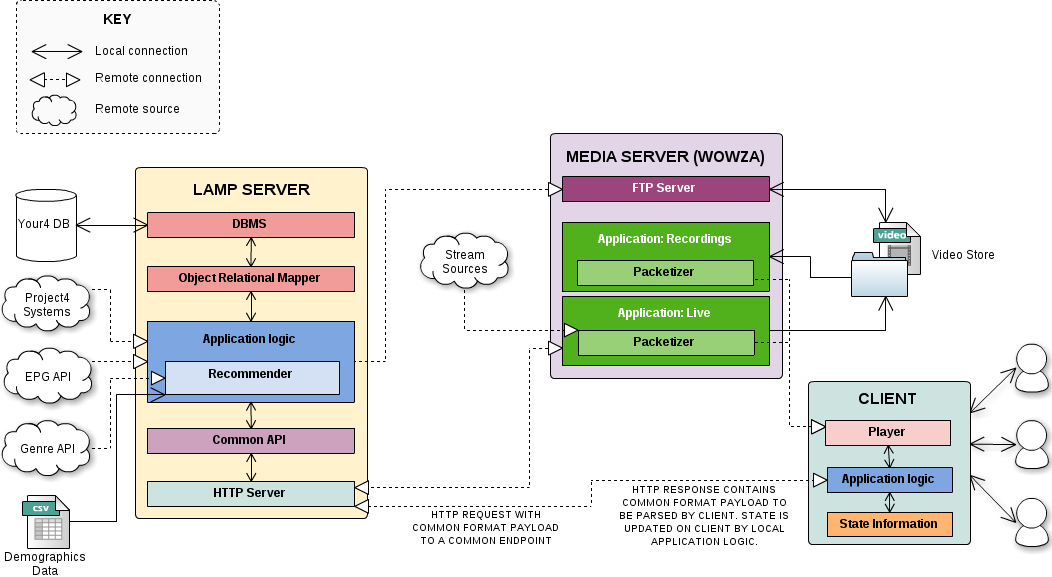
\includegraphics[width=\textwidth]{images/your4-architecture.png}
	\caption{Overview of Your4 architecture}
	\label{fig:your4-architecture}
\end{figure}

Figure~\ref{fig:your4-architecture} shows the overall architecture of the Your4 system. The system is split into three distinct parts:

\begin{description}
	\item[Client:] The client (expected to be Mobile Safari for iPad running on iOS 5+) is responsible for for interfacing with the LAMP server to retrieve the users' personalised playlist. With this playlist, the player in the client can then request the appropriate media from the media server.
	\item[LAMP server:] The LAMP server represents the bulk of the system itself and is responsible for providing a REST API for the key features of Your4: recommendations, user authentication, Electronic Programme Guide (EPG) data and advert uploading and manipulation.
	\item[Media server:] The media server is responsible for encoding and serving live streams as well as recording programmes and serving recorded programmes.
\end{description}

\subsubsection{Client}

The client receives all HTML content from the LAMP server upon the first visit to \textit{Your4.tv}. From this point onwards, all communication between the client and LAMP server contain only models and collections (e.g. a programme and all of its attributes) on the LAMP server's REST interface in JSON format. The client side application is then responsible for parsing this JSON response and manipulating the user interface using local templates (embedded in the HTML during the initial page load) as appropriate. Due to the asynchronism this approach brings, a significant UI speed increase can be observed against traditional methods whereby the web browser acts as a ``thin client'', simply parsing and rendering HTML responses that are pre-generated server side.

Using the POST, GET, PUT and DELETE methods in HTTP requests to the REST endpoint maps to the equivalent create, read, update and delete (CRUD) operations on the object concerned. This methodology creates a simple, self-documenting API. In a similar exploitation of HTTP philosophies, standard HTTP status codes are used to identify the status of a request. For example, 200 indicates success and 400 indicates the request was invalid (failed server side validation). The client can then perform the appropriate callback function to manipulate the object interface.

\paragraph{Authentication}

The concept of a ``user'' is key to the system since crucial demographics data and matrices defining recommender state are stored against each user. The client authenticates a user by either local login or using the Facebook login API\footnote{Facebook API documentation -- \footurl{https://developers.facebook.com/docs/concepts/login}}. During page load, the client attempts to retrieve \texttt{/api/users/me} from the server to discover if an active session is available. If so, the stream player layers will be rendered on screen, otherwise, the user will be first routed to the login interface.

The user can then choose to use the local login which will generate a GET request with the email and password as query parameters. If a HTTP 200 response is received, the login is considered to be successful. A user can alternatively choose to login via Facebook. After the user accepts the Facebook permissions, a local cookie is set and a GET request is generated to \texttt{/api/users/fb-[facebook\_id]} where \texttt{[facebook\_id]} is retrieved from the Facebook API.

\paragraph{Playback}

Upon initialisation of the player, a number of layers are rendered to create the visual appearance of the client:

\begin{description}
	\item[Video layer:] The video component receives and renders the stream. If on an Apple device, this is a HTML5 video tag. Otherwise, a Flash video player is instantiated.
	\item[Skip layer:] Contains user controls to skip and rate currently playing media.
	\item[Black layer:] Used occasionally, as a presentation shim to hide buffering video and thereby provide a more seamless streaming experience.
	\item[Overlay layer:] An iframe which displays the HTML advertisers have specified to be overlayed on their advert.
\end{description}

Once rendering is complete, the client requests a number of resources from the REST API in order to compile and play a playlist:

\begin{enumerate}
	\item A list of channels including the relevant stream URL for the media server.
	\item The current LAMP server timestamp. This is used in recommendation requests.
	\item A request is made for the best recommended live broadcast. This recommendation is based on the currently playing program on each channel. Live broadcasts are given priority over recorded programmes as this is close to the ``personal TV channel'' ideal and reduces load on the server (live broadcasts are multicast). The current timestamp and user ID is sent with this request in order for the server to determine what suitable programmes are upcoming. If an HTTP 200 response is received, the body will include the channel ID. If an HTTP 404 is received, no appropriate live broadcast recommendation is available. The client will then request a recorded programme recommendation. In both cases, the response also includes the programme ID from the EPG and the location of ad breaks.
	\item Using the programme ID, a request is made to retrieve the programme data such as name, description and length.
	\item Between each recorded programme a 2 minute advert break is inserted. Up to 5 minutes is allowed between live broadcasts (depending on previous programme end and the start of the live broadcast). The system is also aware of advert breaks in programmes within the playlist. For each advertisement break, a request is made containing the user ID; programme ID; the amount of time in the break; whether the advert break is between live or recorded programmes and finally a list of advert IDs which have already been used in the playlist. Using this data, the LAMP server can select adverts that match the users demographics and the currently playing programme. This step is repeated multiple times, reducing the amount of time left unallocated in the request each time, until all ad breaks are full.
	\item Steps 3 to 5 are repeated until the minimum duration and size of playlist are both satisfied. Upon each repeat, the timestamp sent with the request is set to the end time of the previously recommended programme or advert. This informs the recommender as to the point in time it should check live broadcasts for suitable programmes.
	\item The playlist is rendered on screen.
	\item The video player is instructed to play the first stream URL in the playlist. Each time an item in the playlist ends, a signal is triggered which causes the player to play the next stream. Additionally, another recommendation is requested and added to the playlist.
\end{enumerate}

The client checks the user agent string of the browser to determine what format of media to request from the media server. Apple devices require HTTP Live Streaming (HLS) streams while the Flash player alternative requests an RTMP formatted stream.

\subsubsection{LAMP server}

The LAMP server's primary responsibility is to expose all required functionality on a single REST endpoint, \texttt{/api}. In general, the LAMP server deals with a request by passing it through various stages before finally manipulating the database:

\begin{enumerate}
	\item An HTTP request is retrieved by the web server.
	\item The request is passed to the REST API where the appropriate function is called dependant on the request URI and HTTP method.
	\item The object in the request body is passed into the Object Relational Mapper.
	\item The ORM builds the appropriate SQL query and passes it to the DBMS.
	\item The DataBase Management System modifies or retrieves from the data store.
	\item The application logic returns the result as an HTTP response containing a JSON-formatted body.
\end{enumerate}

\paragraph{Authentication}

Upon registration, the name, email, gender, date of birth, occupation, postcode and password of the user are required. For Facebook logins, a Facebook ID is required in place of the password. Passwords are stored with a Blowfish-based hash type with a per-user 22 character salt and a 1024 iteration cost parameter which prevents rainbow table exploitation in a human lifetime \citep{hashing}. The postcode is converted to latitude and longitude coordinates based on Ordnance Survey data. Upon successful authentication, a session cookie is created.

A recommender function is also called which retrieves the user's initial genre vector. This is based upon the required demographics data provided at registration. This vector is then stored agaist the user in the database.

\paragraph{Programme recommendations}

EPG data is imported from the Atlas API\footnote{Atlas API website -- \footurl{http://atlas.metabroadcast.com}} into the Your4 database daily. This contains unique programme IDs, descriptions, start and end times, episode numbers, and other programme data.

Upon first initialisation of the recommender, a CSV file containing training data from the GroupLens research group\footnote{GroupLens website -- \footurl{http://www.grouplens.org/node/73}} is processed. This gives the recommender an initial estimate as to what type of users prefer what genres. During execution of the EPG cron job, each programme is passed to a recommender function to retrieve the initial programme vector to store against it. This function calls the genre API, TVDB\footnote{TVDB API website -- \footurl{http://thetvdb.com}}, to identify this vector. The programme vector stores binary values whereby each position represents a predefined genre. A ``\texttt{1}'' at a particular position indicates that the programme belongs to the genre represented by that position.

Upon receiving a live recommendation request, the recommender selects programmes starting within the next 5 minutes of the timestamp contained in the request (see step 3 in the previously listed playback steps). The recommender then filters out programmes the requesting user has already viewed in the past, and selects the best one according the recommender output. If no suitable live recommendation can be made, a HTTP 404 status code will be returned and the client will request a recorded programme. The recommender then executes a similar process to the live request, but filters programmes by those which have been recorded by the media server.

When a user rates a programme on the client, a request is received by the recommender. This rating is a 5-star system which maps to -1, -0.5, 0, 0.5 and 1 respectively. Upon this request, the recommender tunes the user's vector accordingly. The act of rating also adds the programme to the list of already viewed programmes for a user.

\paragraph{Adverts}
\label{sec:lamp-adverts}
Inqb8r's Project4 hardware systems receive XML data pertaining to the times ad breaks are positioned during programmes as shown in Appendix~\ref{Project4EventFlow}. The information (known as MOS records) is also stored in the Project4 MySQL database. Disregarding network delays, we are potentially able to discover the existence of advertisement breaks up to 1 minute and 8 seconds before they are shown. This information is imported live into the Your4 database and made available via the REST interface. With this data, the client is able to know at which points in time it should request an advert to replace the adverts provided in stream by the broadcaster.

When an advertiser uploads an advert to Your4, an FTP session is instantiated by the LAMP server to the media server. The advert is then uploaded to the media server where it is stored alongside other adverts and recorded programmes in the video store. An interactive overlay can also be specified, which will be used in the body of the iframe element of the overlay layer during playback. Campaign information such as target locations, programmes, gender, age and other specifics can also be specified for storage against the advert in the Your4 database. The advertiser can also specify the times of day (on a per-day basis) and the programmes that they wish their advert to be shown in.

When the client requests an advert, the duration the advert must fill and the IDs of adverts that have already been scheduled in the ad break are included in the request. The LAMP server then performs a search on the database for adverts that match these characteristics (duration less than or equal to the advert break time remaining, and the advert has not been shown already in this break) and the targeting criteria set by the advertiser. Any adverts the user has rated negatively in the past will also be filtered out.

Views, clicks and skips are recorded by the client and feedback is sent to the REST interface. The advertiser can then view these statistics in a dedicated web interface.

\subsubsection{Media server}

Video streams are delivered to the client via a Wowza media server\footnote{Wowza Media Server Website -- \footurl{http://www.wowza.com/}}, hosted on a Windows Server 2008 machine. This resource is provided by Inqb8r, who have extensive experience with Wowza based systems.

The Wowza server is configured to act as a repeater, re-broadcasting the streams provided by Inqb8r. This server is based on two distinct applications. The first application is a custom Wowza module responsible for retrieving the source live streams and relaying these to the client. The second is responsible for streaming recorded programmes and adverts from the video store to the client (the standard Wowza extension ``vod'' allows any file of a valid format in a given directory to be streamed). Both applications use a ``packetizer'' which is responsible for encoding the raw input streams to the output requested (HLS for Apple based devices). The packetizer is chosen based on this request, for example, the ``cupertino'' packetizer is used to encode Apple HLS streams distinguished by the \texttt{.m3u8} file extension in the URL.

The custom module is also responsible for recording programmes. The LAMP server's EPG REST interface is continuously polled for any shows due to start within the next minute to retrieve the start and end times of programmes. Using this data, the application records each programme on each channel and stores the resulting media in the video store. This media is stored with a file name which matches that of the unique ID in the EPG. This allows the client to implicitly build the correct video URL to request when a recorded programme recommendation is made. When a recording starts, the application updates the \texttt{recordState} flag of the programme via the REST interface. This flag is updated again when recording is completed. Using the state of this flag, the recommender is able to filter out programmes which have not yet been recorded during recorded programme recommendation. The recordings application can then stream these media files to the client when requested.

Recording requests are processed by the Wowza LiveStreamRecord module in terms of actions on channels rather than explicit recordings. This means that the module imposes a strict limit of only one simultaneous recording per stream. Due to this restriction, whenever a new programme starts any current recording on the channel is stopped before the new recording is started, ensuring mutual exclusion. The end result is a set of video files for each programme stored in the video store.

As every programme is recorded, scalability in terms of storage is an issue. For this reason, recorded videos are removed after a configurable amount of time. First, the recording is removed from further recommendations by setting the \texttt{recordState} flag of the programme to ``\texttt{deleted}'' via the REST interface. After an amount of time equal to the length of the video has passed, the video file itself is removed. This allows any existing viewers of the recording to complete their viewing of the programme before it is made inaccessible.

\subsection{Database structure}

\begin{figure}[H]
	\centering
	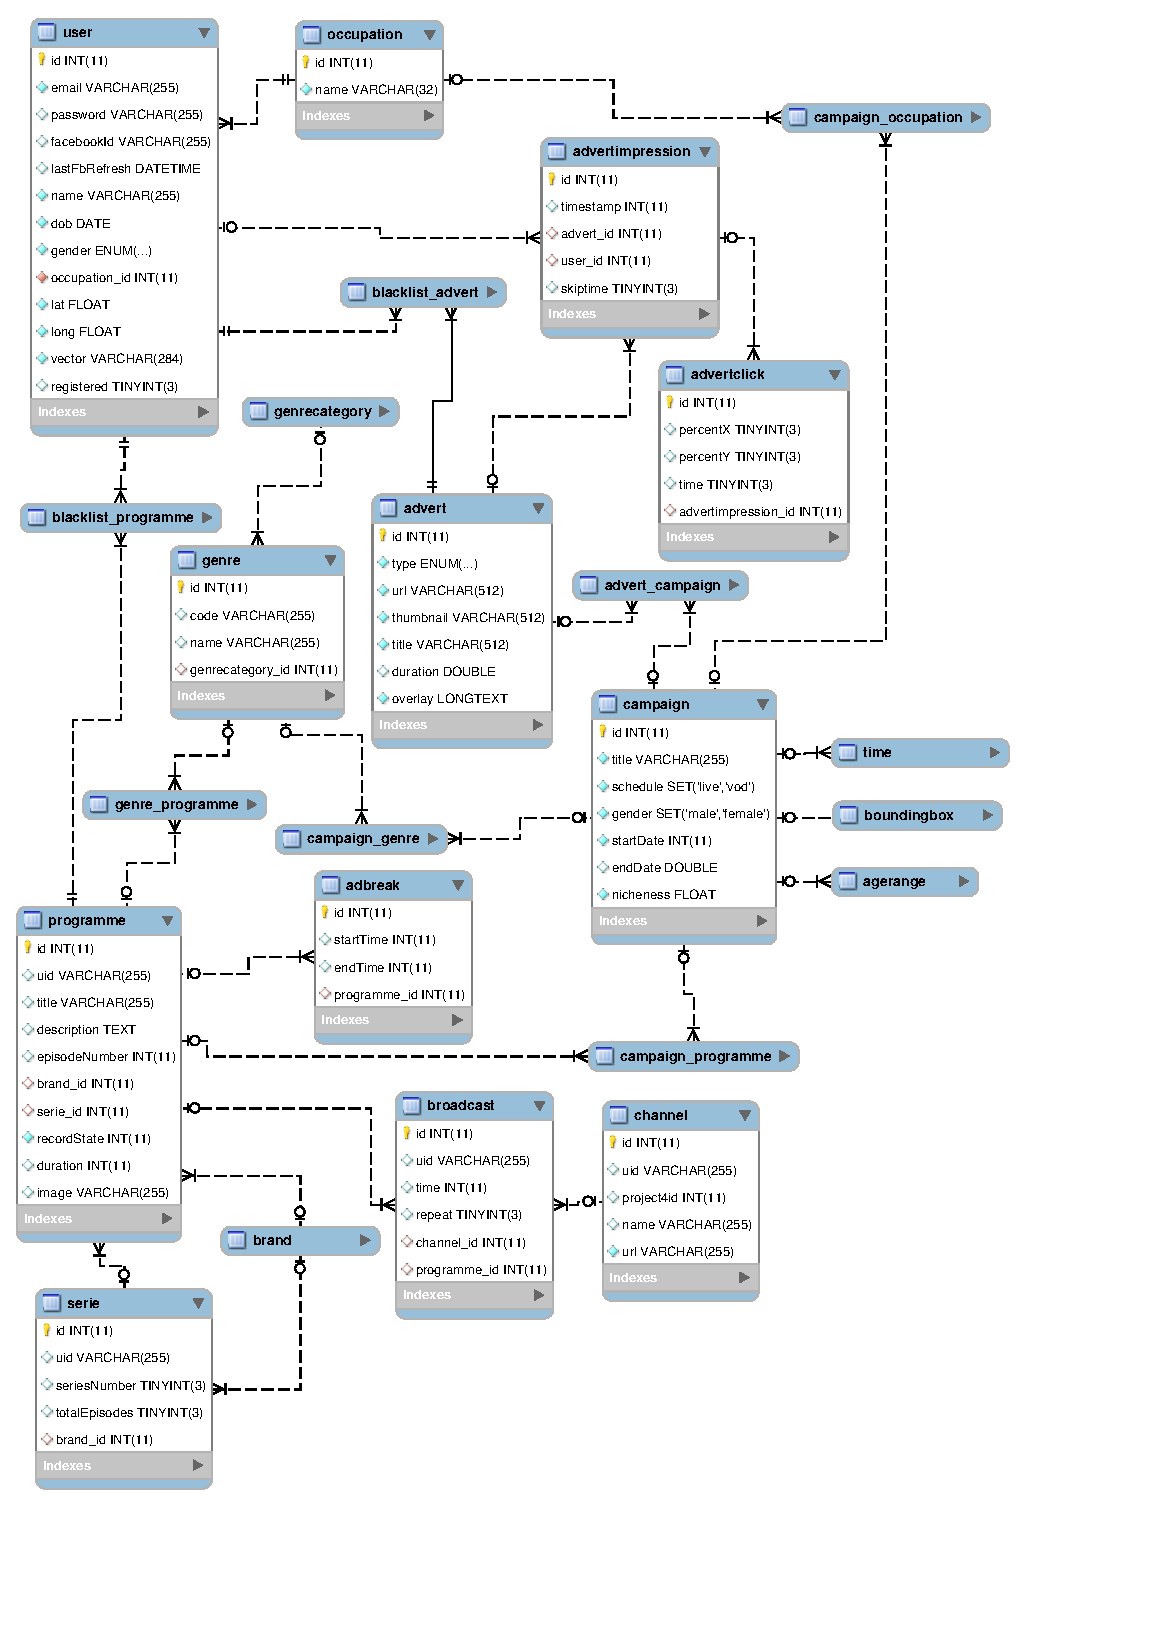
\includegraphics[trim = 0 3.7cm 3.5cm 0, clip, width=\textwidth]{images/your4-db.pdf}
	\caption{Overview of Your4 database layout}
	\label{fig:your4-db}
\end{figure}

Figure~\ref{fig:your4-db} shows the Your4 database class diagram. The Object Relational Mapper (ORM) used enforces a strict naming policy in which all table and attributes are in lower case and are not pluralised. The underscore character represents a relation, e.g. \texttt{programme\_id} represents a foreign key to the \texttt{id} attribute in the programme table.

\subsection{Programming techniques and languages}

The implementation consists of a number of subsystems using different programming languages. The client is built on JavaScript, HTML and CSS; the LAMP server on PHP for the REST interface and Python for the recommender; and finally, the media server is based on a Java implementation. In order to achieve a concise and maintainable solution, a combination of design strategies and good use of libraries was employed.

\subsubsection{Code statistics}
\label{sec:implementation_code_stats}
Table~\ref{tab:metrics} shows the number of lines broken down by language throughout the implementation.
\nopagebreak
\begin{table}[H]
	\centering
	\begin{tabular}{l r r r}
		\toprule
		\textbf{Language} & \textbf{Files} & \textbf{Comments} & \textbf{Code} \\
		\midrule
		JavaScript & 11 & 55 & 2686 \\ 
		PHP & 26 & 28 & 1515 \\ 
		Python & 17 & 282 & 1239 \\ 
		Java & 20 & 322 & 1056 \\ 
		CSS & 5 & 18 & 603 \\ 
		HTML & 2 & 8 & 462 \\ 
		XML & 4 & 100 & 151 \\ 
		\midrule
		sum & 85 & 681 & 7714 \\ 
		\bottomrule
	\end{tabular}
	\caption{Number of lines in Your4 code base}
	\label{tab:metrics}
\end{table}

\subsubsection{Design strategies and patterns}

Where possible, it is good practice to use popular design strategies and patterns as templates to solve common problems in application development. A number of such strategies were used during the implementation stage, the most prevalent of which are documented here:

\begin{description}
	\item[MV*:] By separating models and views using the client-side Backbone.js library, the client is easily able to retrieve objects (models) from the REST interface and attribute them to a view. The view can then use the attributes of the model to render the appropriate HTML in the DOM. This view can also handle user manipulation and edit the models attributes. Models can be swapped in and out of a view easily, and the result re-rendered on screen using Views.
	\item[Front controller:] By using a client-side URL router, navigation is controlled by a single object. This allows for easy tracking and manipulation of the current application navigation state. This router then calls the appropriate function relevant to the currently visited route.
	\item[Observer pattern:] By allowing objects to subscribe to and trigger events, signals can be passed to an object or set of objects without tight coupling. For example, a signal is sent to the player view when an item in the playlist is due to start. As well as the player view, the views representing the playlist are also subscribed to the event, so they can shift the ticker (representing time elapsed on the playlist) to the start of the next programme.
	\item[Fa\c{c}ade pattern:] The LAMP REST interface maps HTTP methods to the equivalent CRUD operations on the object contained within the request body. By providing this self-documenting ``fa\c{c}ade'', the inner complexities and domain-specific operations are hidden from the external API.
\end{description}

\subsubsection{Libraries and frameworks}

A number of libraries and technologies were used during the implementation stage:

\begin{description}
	\item[Client:] \hfill
		\begin{description}
			\item[JQuery:] JQuery allows simple DOM manipulation and event handling.
			\item[Underscore:] A JavaScript library which introduces functional programming aspects with significant performance benefits.
			\item[Backbone:] A Model-View-* framework to interface with REST services.
			\item[Flowplayer:] The Flash player used for non-Apple devices.
			\item[Bootstrap:] A CSS framework defining sensible cross-browser styling.
			\item[D3.js:] Visualisation library which provides graphing capabilities (SVG manipulation).
			\item[Leaflet:] Mapping library with support for mobile touch screen devices.
			\item[Facebook SDK:] Used for Facebook login functionality.
		\end{description}
	\item[LAMP Server:] \hfill
		\begin{description}
			\item[MySQL:] Relational DBMS for primary storage.
			\item[Slim:] PHP framework used to implement REST interface and application logic.
			\item[RedBean:] PHP Object Relational Mapper for easy database manipulation.
			\item[Facebook SDK:] Used for validating Facebook logins.
			\item[TVDB:] Used by the recommender to retrieve programme genres.
			\item[NumPy:] Used by the recommender for manipulation of matrices.
		\end{description}
	\item[Media Server:] \hfill
		\begin{description}
			\item[Wowza:] Multifunctional Java media server.
			\item[LiveStreamRecord:] Wowza module to allow recording of live streams to files.
			\item[Gson:] Java library used to convert objects to and from JSON for the REST interface.
		\end{description}
\end{description}

\subsection{System walkthrough}
\begin{figure}[th]
	\centering
	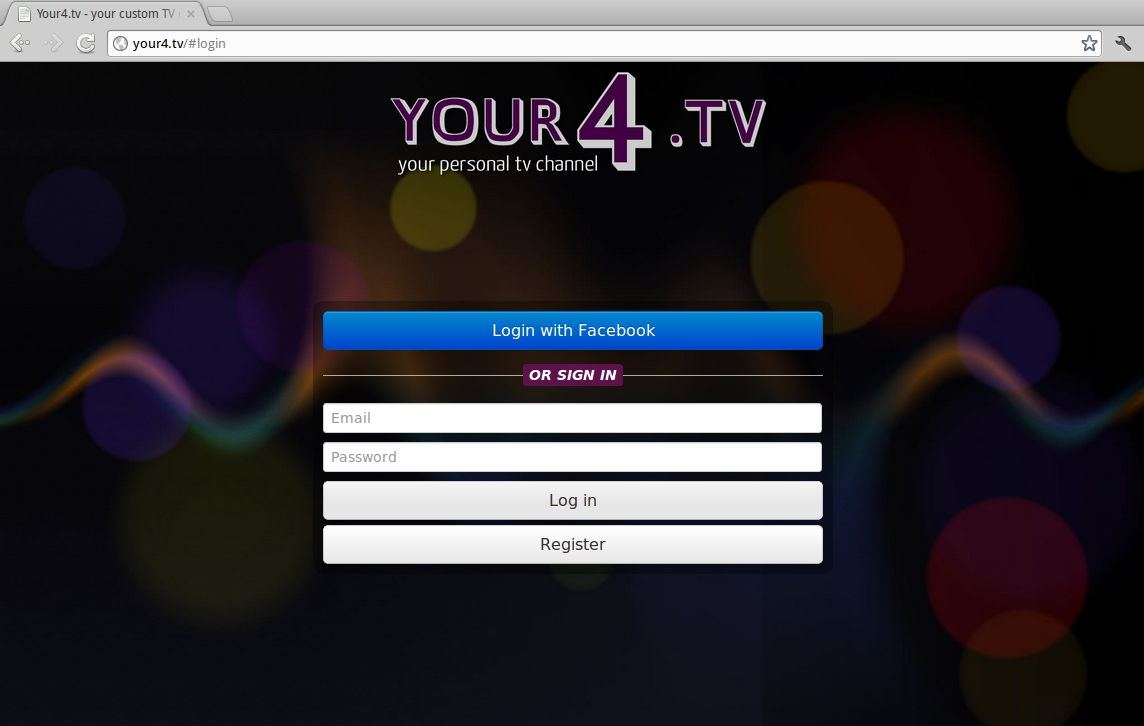
\includegraphics[width=\textwidth,height=0.5\textheight,keepaspectratio]{images/screenshots/your4-login.png}
	\caption{Logging in.}
	\label{fig:your4-login}
\end{figure}
\begin{figure}[th]
	\centering
	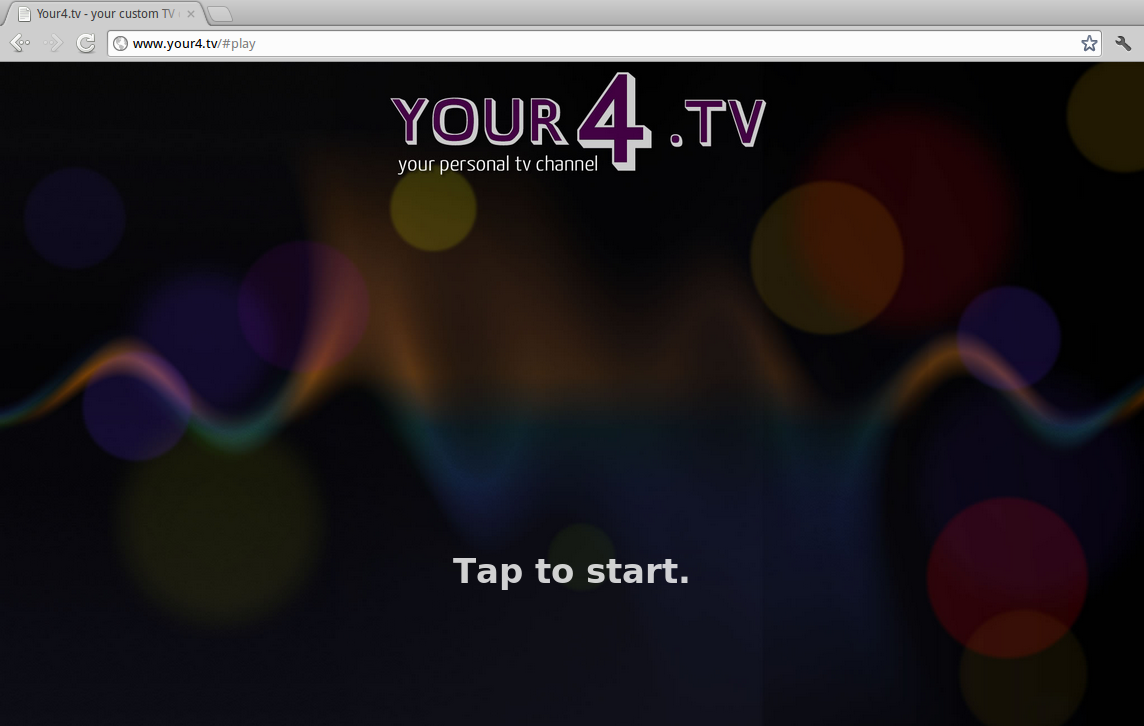
\includegraphics[width=\textwidth,height=0.5\textheight,keepaspectratio]{images/screenshots/your4-tap-to-start.png}
	\caption{Video playback is started by capturing a touch event and relaying a trigger to the video element.}
	\label{fig:your4-tap-to-start}
\end{figure}
\begin{figure}[th]
	\centering
	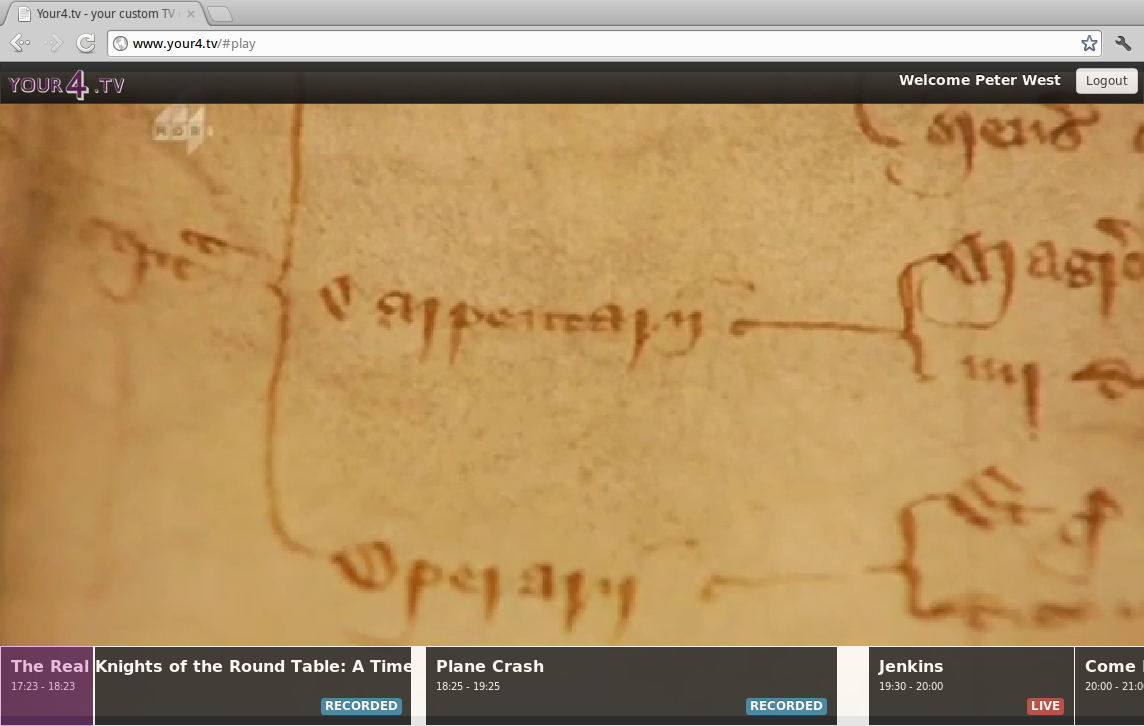
\includegraphics[width=\textwidth,height=0.5\textheight,keepaspectratio]{images/screenshots/your4-play.png}
	\caption{The playlist is shown when the user taps the screen. It slides out of view after a few seconds. It can be scrolled by dragging left and right to view more items.}
	\label{fig:your4-play}
\end{figure}

\begin{figure}[th]
	\centering
	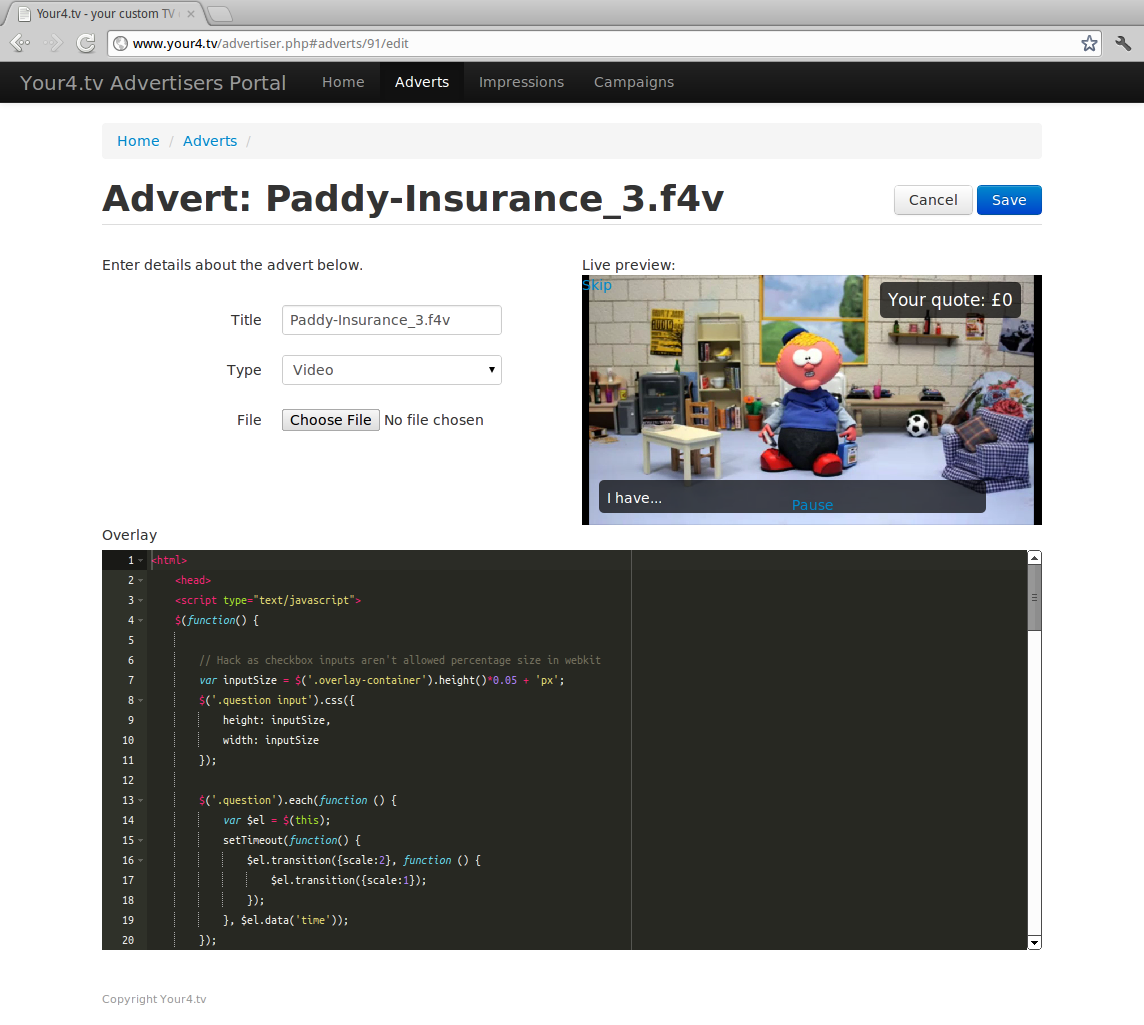
\includegraphics[width=\textwidth,height=0.5\textheight,keepaspectratio]{images/screenshots/advertiser-advert-edit.png}
	\caption{Advertisers can preview their advert overlays and edit them with full syntax highlighting.}
	\label{fig:advertiser-advert-edit}
\end{figure}
\begin{figure}[th]
	\centering
	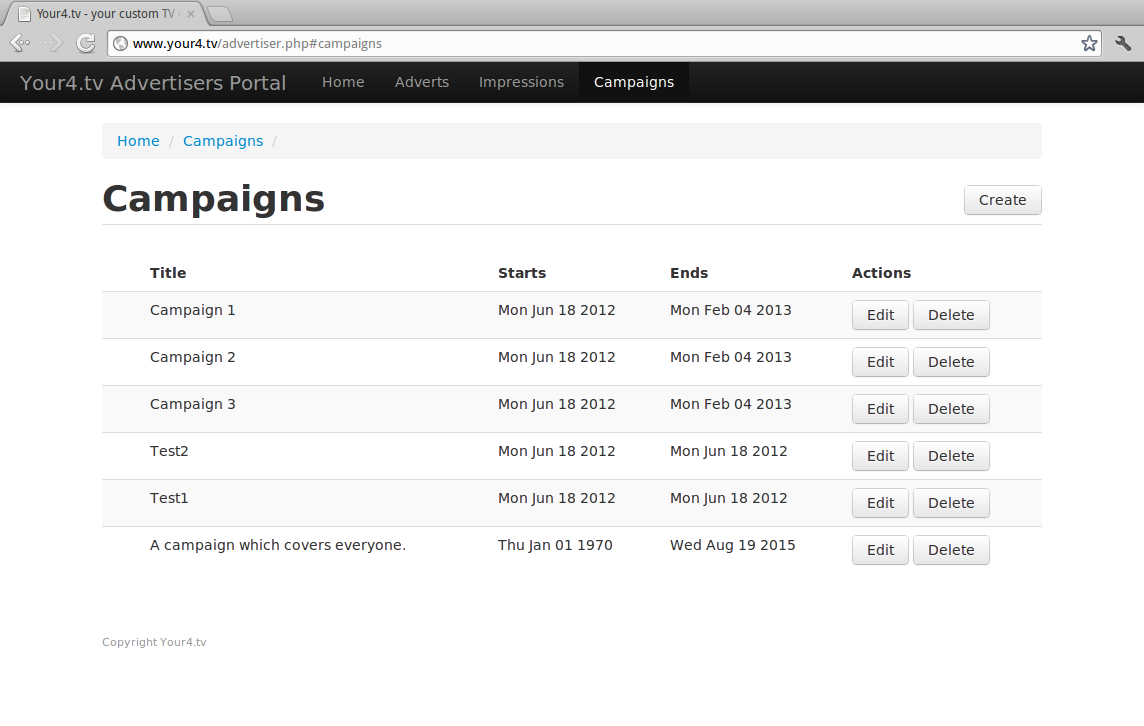
\includegraphics[width=\textwidth,height=0.5\textheight,keepaspectratio]{images/screenshots/advertiser-campaigns.png}
	\caption{Advertisers can view the adverts attached to their campaigns.}
	\label{fig:advertiser-campaigns}
\end{figure}
\begin{figure}[th]
	\centering
	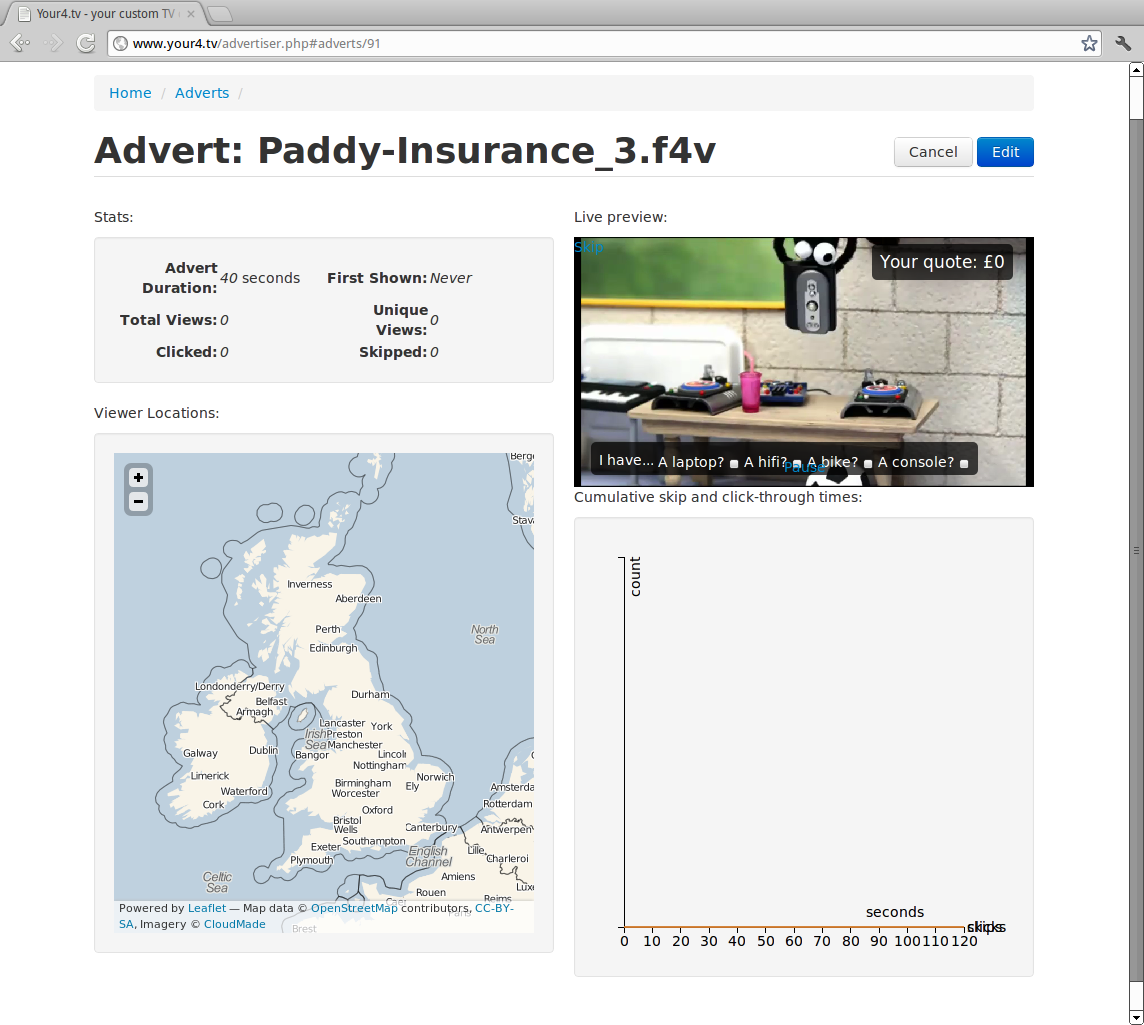
\includegraphics[width=\textwidth,height=0.5\textheight,keepaspectratio]{images/screenshots/advertiser-advert.png}
	\caption{Statistics can be viewed pertaining to an advert.}
	\label{fig:advertiser-advert}
\end{figure}
\begin{figure}[th]
	\centering
	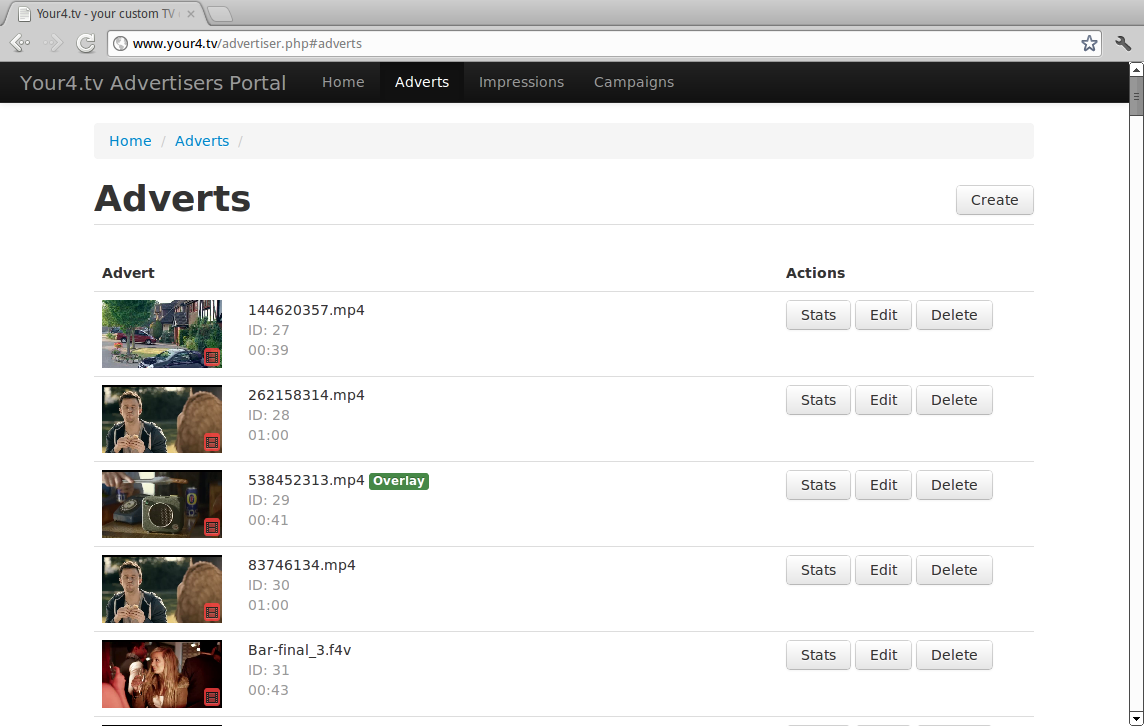
\includegraphics[width=\textwidth,height=0.5\textheight,keepaspectratio]{images/screenshots/advertiser-adverts.png}
	\caption{Advertisers can view and remove their adverts.}
	\label{fig:advertiser-adverts}
\end{figure}
\begin{figure}[th]
	\centering
	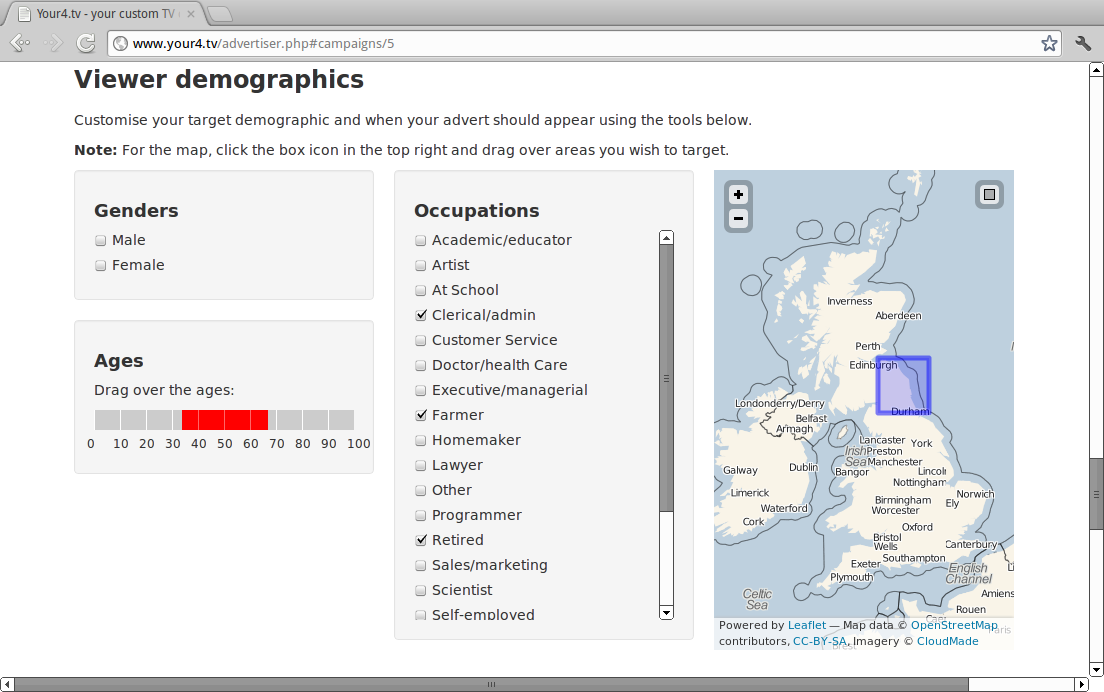
\includegraphics[width=\textwidth,height=0.5\textheight,keepaspectratio]{images/screenshots/advertiser-campaign-demographics.png}
	\caption{Advertisers can specify the target demographics for their campaigns.}
	\label{fig:advertiser-campaign-demographics}
\end{figure}
\begin{figure}[th]
	\centering
	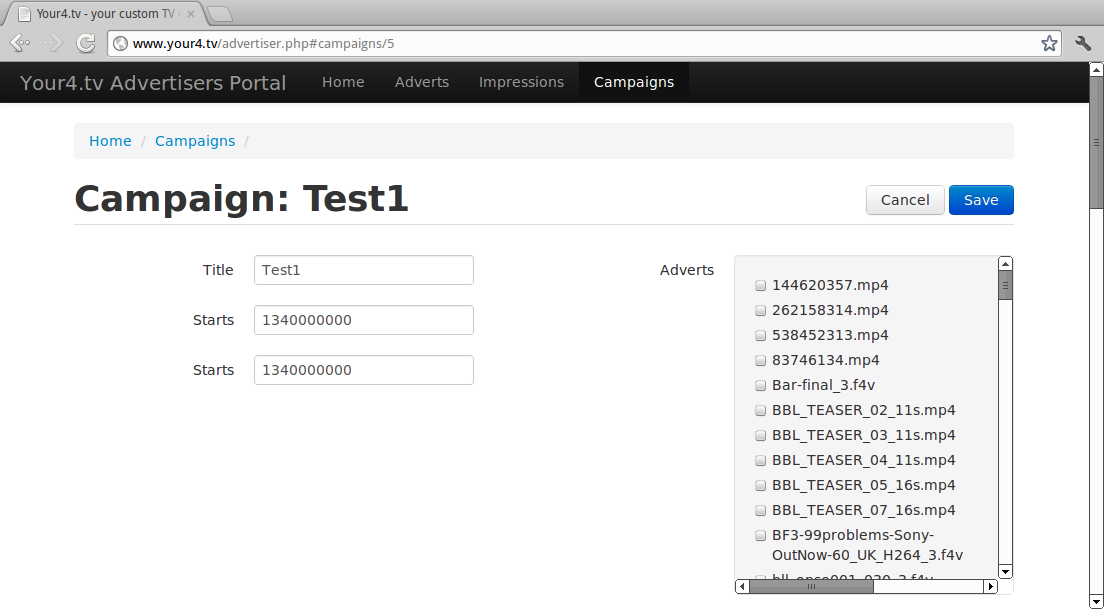
\includegraphics[width=\textwidth,height=0.5\textheight,keepaspectratio]{images/screenshots/advertiser-campaign.png}
	\caption{A campaign is attached to an advert.}
	\label{fig:advertiser-campaign}
\end{figure}
\begin{figure}[th]
	\centering
	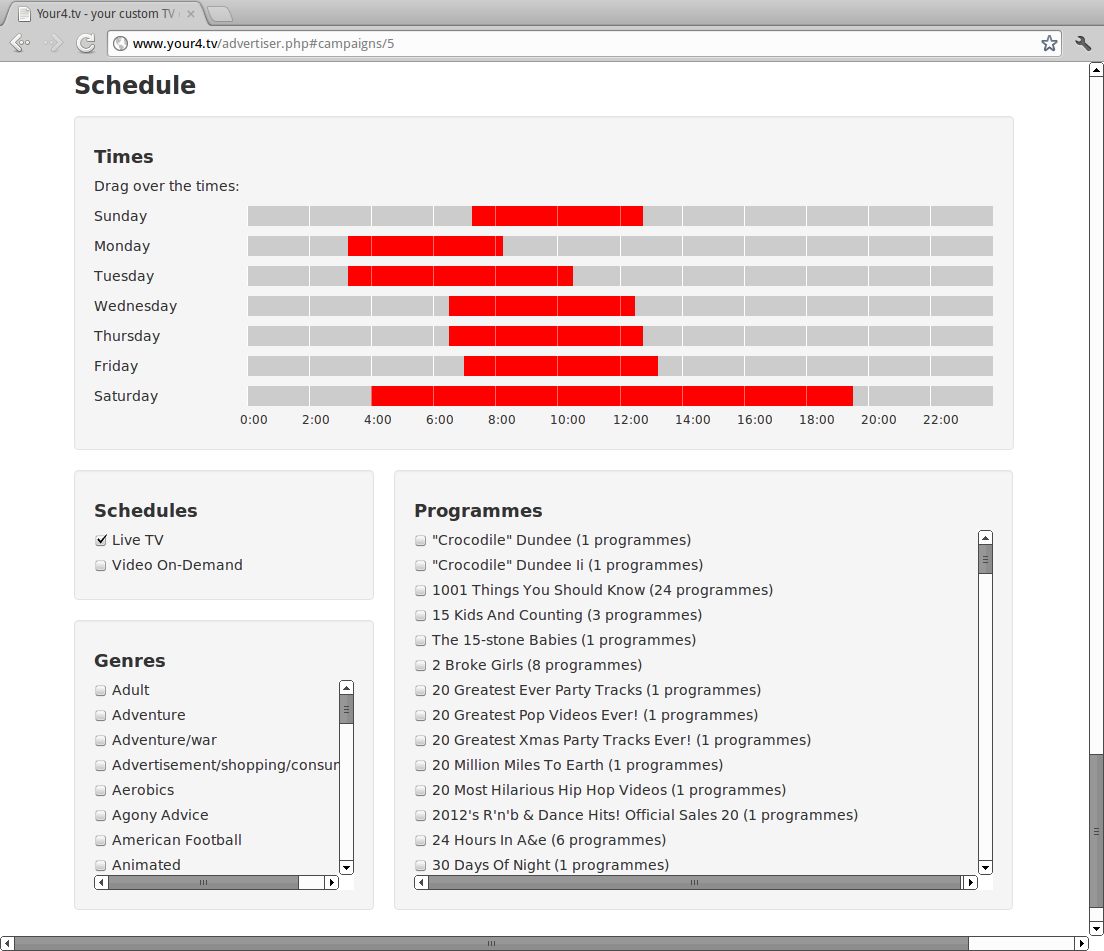
\includegraphics[width=\textwidth,height=0.5\textheight,keepaspectratio]{images/screenshots/advertiser-campaign-schedule.png}
	\caption{Campaigns can be scheduled during specific weekdays and attributed to specific genres or programmes.}
	\label{fig:advertiser-campaign-schedule}
\end{figure}
